\subsection[Architektura środowiska testowego]{Architektura środowiska testowego}
\begin{figure}[H]
    \centering
    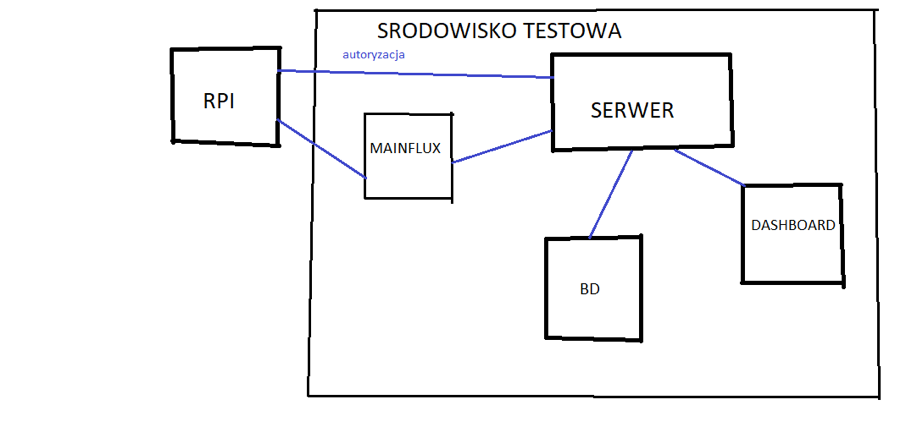
\includegraphics[width=\textwidth]{kp01}
    \caption{Schemat przedstawiający podstawowe zależności w środowisku testowym } % role Środowiska testowego w dedykowanym systemie
    \label{fig:iotarch}
\end{figure} 
Środowisko testowe składa się z kilku komponentów programowych: aplikacji sterującej, platformy Mainflux, bazy danych, dashboardu oraz klienta komunikacji. Wszystkie wymienione elementy za wyjątkiem klienta komunikacji znajdują się na jednej maszynie.
Aplikacja sterująca to oprogramowanie, które ma kilka zadań do spełnienia. Pierwszym jest zapewnienie autoryzacji platformy wykonującej. Każda platforma jest skonfigurowana w Mainfluxie jako \textit{rzecz} (opisana rozdziale~\ref{subsection:wp}). Posiada swój zewnętrzny identyfikator oraz klucz. W momencie, gdy platforma wykonująca chce otrzymać swoje dane (tzn. klucz rzeczy, identyfikator rzeczy oraz 2 przypisane kanały) wysyła żądanie HTTP na serwer z zewnętrznym identyfikatorem oraz kluczem. Platforma wykonująca potrzebuje 2. kanałów, ponieważ na jednym będzie nadawać wiadomości, a na drugim odbierać. Aplikacja sterująca po otrzymaniu zapytania sprawdza czy zewnętrzny identyfikator, przesłany przez platformę wykonującą, znajduję się już w bazie danych, jeśli tak to pobiera jego dane oraz zwraca je. W przeciwnym razie aplikacja sterująca dzięki Mainflux CLI loguje się jako administrator, tworzy nową rzecz oraz 2 kanały, po czym przypisuje je do stworzonej rzeczy oraz do rzeczy serwera. Rzecz serwera jest to specjalny obiekt, który ma przypisane do siebie wszystkie kanały i jest tworzony przy starcie środowiska testowego. 
Kolejnym zadaniem aplikacji sterującej jest przesyłanie wiadomości z panelu użytkownika na platformę wykonującą oraz odbieranie od niej wiadomości. Wysyłanie wiadomości jest stosunkowo łatwe. Wystarczy, że aplikacja sterująca wyśle ładunek na odpowiedni kanał. Odbieranie jest bardziej skomplikowane. Aplikacja sterująca musi stale nasłuchiwać na danym kanale. Ze względu na to, że wiele platform wykonujących może w tym samym momencie wysyłać wiadomości, aplikacja powinna jednocześnie nasłuchiwać na wszystkich kanałach. Do listy nasłuchiwanych kanałów dodawane są te, które znajdują się w bazie danych. Oznacza to, że w momencie gdy nowa platforma wykonująca przechodzi proces autoryzacji, listę należy odświeżyć.


Aplikacja sterująca oferuje rest api, które udostępnia metody potrzebne do stworzenia Dashboardu. Dashboard jest to łatwy w odczycie interfejs, który pośredniczy miedzy pentesterem a aplikacją sterującą. 
Jednym z jego celów jest wyświetlenie wiadomości przesłanych przez platformę wykonującą. Pozwala to pentesterowi na przeglądanie wiadomości. 
Interfejs użytkownika wyświetla również aktywne platformy wykonujące. Aplikacja sterująca udostępnia (wykorzystując rest api) listę aktywnych urządzeń. Jest ona uaktualniana co 5 sekund. % Dane na ich temat, znajdują się na liście aktywnych urządzeń i są umieczszone w aplikacji sterującej.
Uaktualnianie polega na tym, że platforma wykonująca co 2s zgłasza aktywność, jeśli serwer nie otrzyma wiadomości od platformy przez więcej niż 4s aktualny wynik zostaje usunięty. 
Dashboard umożliwia wysłanie ładunku na wskazaną platformę lub do wszystkich aktywnych urządzeń. %Serwer pozwala na wysłanie wiadomości na wskazaną platformę lub do wszystkich aktywnych urządzeń. 
Wysłanie ładunku na pojedynczą platformę wymaga podania zewnętrznego identyfikatora urządzenia. 
Serwer po otrzymaniu zapytania sprawdza, czy wskazane urządzenie istnieje. Jeśli tak to pobiera kanał, na którym nasłuchuje oraz wysyła wiadomość. 
Jeśli pentester chce wysłać ładunek do wszystkich platform wykonujących, to musi w polu przeznaczonym na identyfikator wpisać słowo \textit{All}. 
Serwer pobierze wtedy listę aktywnych urządzeń oraz wyśle wiadomości na przypisane do nich kanały. 
Otrzymane odpowiedzi można przeczytać na liście przesłanych wiadomości.
Opisane ST zostało wykorzystane do zapewnienia pentesterowi stałego dostępu do platform wykonujących oraz zdalnego wykonywania testów. 
Sposób użycia ST został przedstawiony w scenariuszach \textit{Podszywanie pod HID}, \textit{Pharming} i \textit{Mitm} (rozdziały~\ref{sce:klawiatura}, \ref{sce:phar} i~\ref{sce:mitm}).
\begin{figure}[H]
    \centering
    \fbox{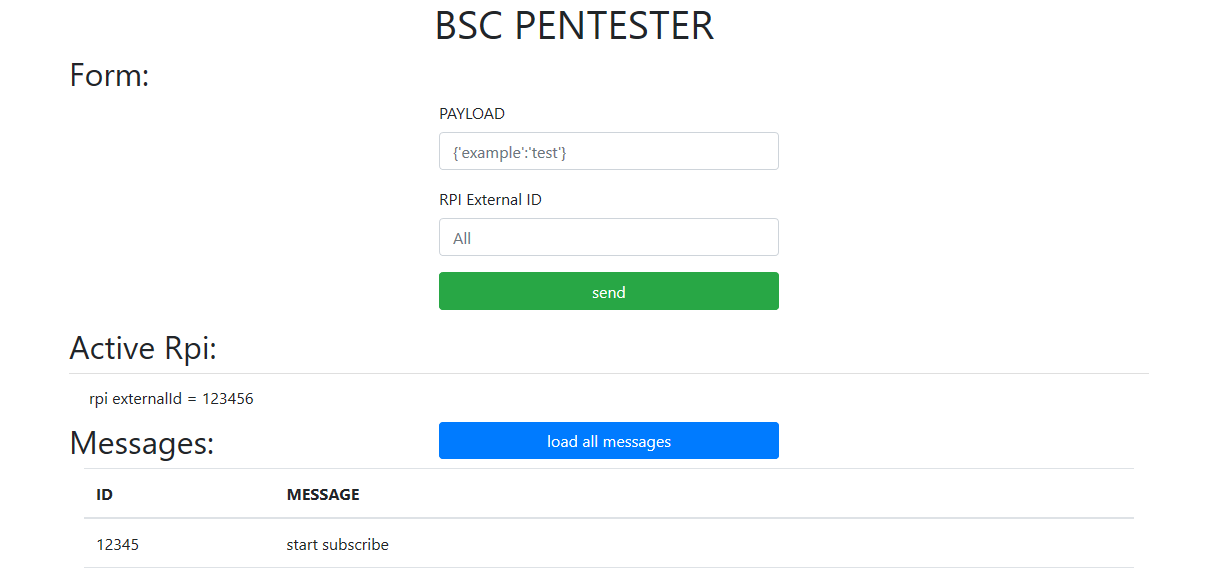
\includegraphics[width=0.95\textwidth]{kp09}}
    \caption{Zrzut ekranu - interfejs pentestera}
    \label{fig:dahsboard}
\end{figure}